

%\chapter*{Appendix}
%\markboth{Appendix}{Appendix}
%\addcontentsline{toc}{chapter}{Appendix}
%\setcounter{chapter}{1} 

%\appendixname{Appendix}



\chapter{Software, data, collaborations}
\label{sec:availability}

I follow the principles of Open Science as I am convinced they make research more transparent: 
\begin{itemize}
\item I make my dissertation thesis and all scientific publications, to which I refer to, \textbf{open access}.
\item I make the software \textit{CrowNet} \textbf{free and open source}. I use this software in my studies.
\item I make my simulation \textbf{data open}. This includes raw data, post-processing scripts, and the actual results.
\item I foster \textbf{collaboration} with experts from different fields.
\item I ensure the \textbf{reproducibility} of my data.
\end{itemize}
I guarantee that my data and source code is at least available until 01.01.2035. For storing these, I use \textit{LRZ sync and share} and \textit{github}.




\subsubsection*{Simulation data and software}
The results of my simulation studies (sections~\ref{sec:investigation}) are publicly available via \textit{LRZ sync and share}:
\begin{itemize}
\item  Raw data (57\,GB). Includes trajectories, database with mobile communication recordings, etc. \url{https://syncandshare.lrz.de/getlink/fiTUk3Xso5YSpLezh5dXXR/rawdata-2023-12-16.zip}. 
\item Output from analysis (0.06\,GB). Includes figures, tables, text files, etc. \url{https://syncandshare.lrz.de/getlink/fiDVxs4LRF2gaD4P4dHDQM/data-2023-12-16-11.zip}
\end{itemize} 
The data was created with the software \textit{CrowNet} developed at hochschule München University of Applied Sciences in Munich, Germany. The software is described in Chapter \ref{sec:crownet}. The data was produced using the stable branch of the software  (stable branch: 15 Dec 2023, git commit hash: 69af8b55bc9f40f21ad32070ee429397635b4d85).
The software is freely available on github: \url{https://github.com/roVer-HM/crownet}. 

\newpage
The 15 Dec 2023 state is freely available
\begin{itemize}
\item  as zip-file (version 69af8b55) via LRZ sync and share (6GB): Contains binaries, virtual environments. \url{https://syncandshare.lrz.de/getlink/fiC254uPj28rFMp2ke1QXG/crownet.zip}
\item {as repository on github (Version 69af8b55)}: Clean repository (requires less storage because it does not contain any binaries or virtual environments). \url{https://github.com/roVer-HM/crownet/commit/69af8b55bc9f40f21ad32070ee429397635b4d85}
\end{itemize} 
Three Docker images are used in the simulation studies: one for each of the simulators \textit{Vadere, flowcontrol and OMNeT++}. The Docker images are publicly available
\begin{itemize}
\item through the image registry of the \textit{CrowNet} repository on github: \url{https://github.com/orgs/roVer-HM/packages?repo_name=crownet}. You can simply download the images by copying the following commands in a terminal:
\lstinline{docker pull ghcr.io/rover-hm/vadere:46c81df1 && docker pull ghcr.io/rover-hm/flowcontrol:496ff02c && docker pull ghcr.io/rover-hm/omnetpp:6.0.1}\textit{}
\item as zip-file on sync and share (3.3\,GB): download the images from  \url{https://syncandshare.lrz.de/getlink/fiY1WxE1p8VoQtHFMCk3K5/dockerimages.zip} and extract the zip-file and restore each image using \lstinline{docker load}. 
\end{itemize}


\subsubsection*{Reproducability of the simulation data}

To reproduce the results of Chapter~\ref{sec:investigation}, please follow the next steps.
First, make sure that your system meets the following requirements:
\begin{itemize}
\item Linux operating system with \lstinline{git} and \lstinline{Docker} installed
\item  $\geq$ 70\,GB available memory
\item  $\geq$ 80 CPUs
\item $\geq$ 170\,GB free disk space for storing the simulation data 
\end{itemize}
Second, run the simulation studies. This comprises cloning the \textit{CrowNet} repository and executing the script 
\lstinline{crownet/scripts/run_simulations_Diss_Mayr}. You can simply do this by pasting the following lines in your terminal:

\begin{lstlisting}[]
$ git clone --recurse-submodules https://github.com/roVer-HM/crownet.git
$ cd crownet && git checkout 69af8b55bc9f40f21ad32070ee429397635b4d85
$ source setup -i 
$ cd scripts && ./run_simulations_Diss_Mayr
\end{lstlisting}
Note that the script checks whether your system fulfills the requirements before the simulation studies are executed. 
Third, wait approximately 14 hours for the simulations to be finished. The script will tell you whether the simulation data has been reproduced successfully.
This procedure was tested on the system described in Appendix~\ref{sec:VirtualMachine}. 


\subsubsection*{Survey data}
\label{sec:surveydata}
The raw data from the online survey (see Section \ref{sec:reaction}), as well as analysis scripts and results of statistical tests are freely available
\begin{itemize}
\item {as zipped repository via LRZ sync and share (0.5MB)}:  \url{https://syncandshare.lrz.de/getlink/fiWz7mx6v8ZG7mCu2UKvi6/survey-route-choice-master.zip}
\item {on github}: \url{https://github.com/pedestrian-dynamics-HM/survey-route-choice} (github repository)
\end{itemize} 

To reproduce the results, please clone or download the repository and run the scripts in the root directory. This requires R to be installed. I tested the scripts for R version 3.6.3 (2020-02-29) on a Linux operating system (Ubuntu 20.04).


\subsection*{Collaboration with other scientists}
\label{sec:collaboration}
Some parts of this work have been developed in collaboration with other scientists. I would like to acknowledge their contributions in the following.

\subsubsection{Contributions to the Software \textit{CrowNet}}


\textit{CrowNet} was developed in the \textit{roVer} research project (2018-2023) at Hochschule München Munich University of Applied Sciences (Munich, Germany). 

Stefan Schuhbäck implemented the initial coupling of the simulators \textit{Vadere} and \textit{OMNeT++}~\cite{schuhbaeck-2019-com}. He also introduced the virtualization of the simulators using Docker images. Furthermore, he proposed the decentralized pedestrian density map application~\cite{schuhbaeck-2021-com,schuhbaeck-2023-com}. 

Several others contributed to the source code of \textit{CrowNet}: Prof. Dr. Lars Wischhof (project lead of \textit{roVer}), Sebastian Benz (student), Matthias Rupp (student), Nico Dassler (student), Wolfgang Kallies (student), and Maximilian Kilian (student). I would like to mention them even if I do not use their work in my investigations.

My individual contributions for each \textit{CrowNet} module are: 

\begin{itemize}
\item \textit{flowcontrol} module: I developed the core of the novel Python framework on my own. The core comprises the route recommendation algorithms, the timestepping procedures, and the density mapping. Stefan Schuhbäck supported me with the implementation of the Traffic Control Interface that enables the communication with other simulators. \textit{flowcontrol} is my major contribution to the \textit{CrowNet} software.
\item \textit{SUQ-controller} module: I extended the existing framework \textit{SUQ-controller} (\url{https://gitlab.lrz.de/vadere/suq-controller}) that was developed by Daniel Lehmberg. I added new process calls to execute coupled simulations. 
\item \textit{Vadere} module: I adjusted the existing framework \textit{Vadere} (\url{https://gitlab.lrz.de/vadere/vadere}) so that dynamically generated stimuli can be processed by the psychology layer. The Traffic Control Interface was implemented by Stefan Schuhbäck in~\cite{schuhbaeck-2019-com}.
\item \textit{crownetutils} module: I contributed to the \lstinline{dockerrunner} sub-module. In particular I defined the \lstinline{dockerrunner} for the \textit{flowcontrol} simulator and added methods to start the containers in the correct order.
\item \textit{OMNeT++} module: I did not contribute to this module. The module was developed by Stefan Schuhbäck, Lars Wischhof, and students. 
\end{itemize}
 
\subsubsection{Survey - collaboration with psychologist}

%
In Section~\ref{sec:reaction} I present an online survey. The survey design was developed in collaboration with the crowd psychologist Dr. Anne Templeton (University of Edinburgh, UK). I conducted the survey on my own. I was in charge of storing the data and I conducted the statistical analysis in R. We analyzed results and findings together. 

\subsubsection{Usage of the decentralized density map application}
In Section~\ref{sec:realistiscscenario} I use the decentralized density map application to measure the crowd density in certain areas. The application has been published in~\cite{schuhbaeck-2021-com,schuhbaeck-2023-com} to which I refer to repetitively. 

Nevertheless I would like to briefly describe how the decentralized density map application is related to my work: 
The application is one element of my crowd guidance system. It provides density estimates that are fed into the route recommendation algorithm. I consider the application as a black box because I am interested in the performance of the overall system and not in the performance of individual components. Importantly, my scientific contribution is the assessment of the overall system including the interplay of the density map application and the route recommendation algorithm. 

The density map application is actively researched and further developed by Stefan Schuhbäck with whom I worked together in the \textit{roVer} research project. At the time of writing this thesis, he was further improving the application. These recent developments have not been published yet. Therefore I used an older version of the density map application in my investigations that has been already published in~\cite{schuhbaeck-2021-com,schuhbaeck-2023-com}. 


\subsubsection{Python package omnetinireader}
Stefan Schuhbäck and I developed the \textit{omnetinireader} Python package that is publicly available under:
\url{https://test.pypi.org/project/omnetinireader/1.7.2/}

It serves as external library in the \textit{SUQ-controller} module of the \textit{CrowNet} software.

\clearpage


\chapter{Virtual machine: properties}
\label{sec:VirtualMachine}
I run all simulations on a virtual machine as described in Table~\ref{tab:lscpu} and \ref{tab:memory}.

\begin{table}[hbt!]
\begin{footnotesize}
\begin{tabular}{|p{4cm}|p{10cm}|}
 \hline
Architektur&              x86\_64 \\ \hline
CPU Operationsmodus&     32-bit, 64-bit \\  \hline
Byte-Reihenfolge&        Little Endian \\  \hline
CPU(s)&                  80 \\   \hline
Liste der Online-CPU(s)& 0-79 \\  \hline
Thread(s) pro Kern&      1 \\  \hline
Kern(e) pro Socket&     40 \\  \hline
Sockel&                  2 \\  \hline
NUMA-Knoten&             1 \\  \hline
Anbieterkennung&         GenuineIntel \\  \hline
Prozessorfamilie&        15 \\  \hline
Modell&                  6 \\  \hline
Modellname&              Common KVM processor \\  \hline
Stepping&                1 \\  \hline
CPU MHz&                 2099.998 \\  \hline
BogoMIPS&                4199.99 \\  \hline
Hypervisor-Anbieter&     KVM \\  \hline
Virtualisierungstyp&     voll \\  \hline
L1d Cach&               32K \\  \hline
L1i Cache&               32K \\  \hline
L2 Cache&               4096K \\  \hline
L3 Cache&                16384K \\  \hline
NUMA-Knoten0 CPU(s)&     0-79\\  \hline
Markierungen&           fpu vme de pse tsc msr pae mce cx8 apic sep mtrr pge mca cmov pat pse36 clflush mmx fxsr sse sse2 ht syscall nx lm constant\_tsc nopl xtopology cpuid tsc\_known\_freq pni cx16 x2apic hypervisor lahf\_lm cpuid\_fault pti \\ 
 \hline
\end{tabular} 
\end{footnotesize}
\caption{Virtual machine: processor properties. The following output was generated by calling the terminal command \lstinline{lscpu}\textit{}.}
\label{tab:lscpu}
\end{table}

\begin{table}[hbt!]
\begin{footnotesize}
\begin{tabular}{|p{3cm}|p{1.5cm}|p{1.5cm}|p{1.5cm}|p{1.5cm}|p{1.5cm}|p{1.5cm}|}
\hline
             &  Gesamt    &  belegt  &  frei    &    gemns. & Cache  & verfügbar  \\ \hline
Speicher & 94G & 5,0G & 85G & 145M & 3,7G & 88G \\ \hline
Auslagerungsspeicher&    8,0G    &  0B   &  8,0G  & & &\\ \hline
\end{tabular}
\end{footnotesize}
\caption{Virtual machine: working memory. The following output was generated by calling the terminal command \lstinline{free -h}\textit{}.}
\label{tab:memory}
\end{table}



\newpage

\chapter{Bounds of the control parameter (Section 4.1)}
\label{sec:networkparameters}

The transmitter power parameter should not have an influence in the scenario in Section~\ref{sec:infoverbreitung} if it is in the range the range [2\,mW, 20\,mW]. 


The free path loss formula describes the loss of the signal strength over distance. It is defined as~\cite{friis-1946-com}:

\begin{equation}
\frac{P_{transmitter}}{P_{receiver}} = D_{transmitter} D_{receiver} \left( \frac{4\pi d f}{c} \right)^2
\end{equation}

where $D$ is the antenna directivity which is $D_{transmitter}=D_{receiver}=1$ in my case (isotropic antenna), $d$ is the distance between transmitter and receiver, $f$ is the frequency which is $f=2,4 \cdot 10^9 1/s (= 2.4\,\text{GHz})$, and $c=299 792 358\,\text{m/s}$ is the light speed. The range d is therefore:

%\begin{equation}
%\sqrt{ \frac{P_{transmitter}}{P_{receiver}} } =  \frac{4\pi f}{c}  d
%\end{equation}

\begin{equation}
d = \sqrt{ \frac{P_{transmitter}}{P_{receiver}} }  \frac{c}  {4\pi f}
\label{eq:friis}
\end{equation}

For a transmitter power $P_{transmitter}=2\,$mW and a receiver power of $P_{receiver}=3.16 \cdot 10^{-9}mW (=-85dB)$~\cite{burbank-2011-com} the coverage is $250\,$m according to Eq.~\eqref{eq:friis}. Since the diagonal of the rectangular topography is only $d_\text{max}=213\text{m} (=\sqrt{176\,\text{m}^2+120\,\text{m}^2})$, nodes are always in coverage if the transmitter power is $\in$ [2\,mW, 20\,mW]. See Fig.~\ref{fig:pathlossfriis}.


\begin{figure}[H]
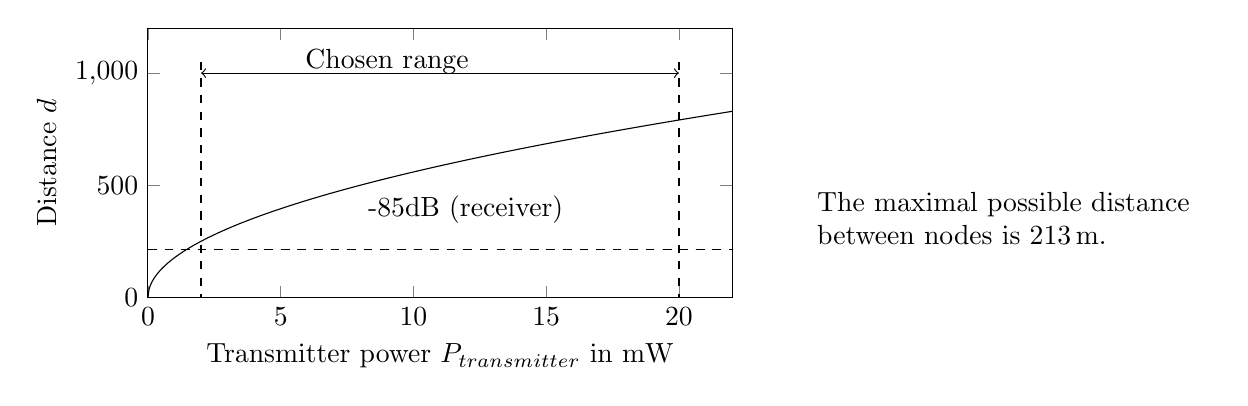
\begin{tikzpicture}
\begin{axis}[
    xmin = 0, xmax = 22,
    ymin = 0, ymax = 1200.0, samples=500, xlabel={Transmitter power $P_{transmitter}$ in mW},
        ylabel={Distance $d$}, height=5cm, width=9cm]
    \addplot[        domain = 0:22
    ] {sqrt(x/0.00000000316)*299792358/(4*pi*2400000000)} node[right,pos=0.6,yshift=-0.3cm]{-85dB (receiver)}; % -85dBm    
      \addplot[dashed, domain = 0:25,] {213} node[right,pos=0.8]{}; % -80dBm
     \draw[<->] (2,1000) -- (20,1000); 
     \draw[dashed] (2,1050) -- (2,0); 
     \draw[dashed] (20,1050) -- (20,0); 
\end{axis}
 \node[text width=5cm] at (11,1) {The maximal possible distance between nodes is 213\,m.  }; 
  \node[text width=5cm] at (4.5,3) {Chosen range }; 

\end{tikzpicture}
\caption[Damping over distance for mobile connections]{Range over the transmitter power according to the formula~\eqref{eq:friis}. The greater the transmitter power, the greater the range. With a transmitter power of 2\,mW, the range is already 250\,m. The maximum distance is 213\,m. Therefore all nodes are in coverage for a transmitter power $>2$\,mW. }
\label{fig:pathlossfriis}
\end{figure}

\chapter{Effect of network traffic (Section 4.1)}
\label{sec:effectofnetworktraffic}
The study presented here is similar to the study in Section~\ref{sec:infoverbreitung} and is based on the publication \cite{mayr-2021-com}. Code and data associated to the study can be found in the repository \url{https://github.com/pedestrian-dynamics-HM/crownet-uq-analysis}.
The scenario of this study is similar to the scenario presented in Section~\ref{sec:infoverbreitung} with three exceptions:

\begin{itemize}
\item the relay node is not shadowed by walls. 
\item network traffic is present. 
\item the arrivals follow an negative exponential distribution. 
\end{itemize} 


\begin{figure}[hbt]
\centering
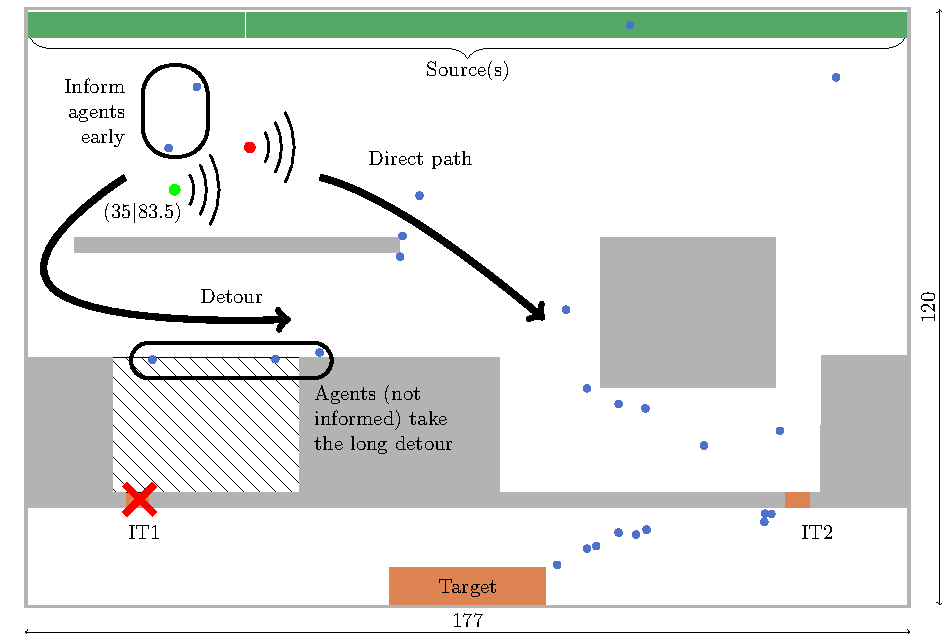
\includegraphics[width=13.5cm]{./appendix/trafficInfluence/Figure10}%
\caption[Scenario for investigating the effect of network traffic]{ Scenario for investigating the effect of network traffic. 
Scenario similar to the scenario introduced in Sec.~\ref{sec:infoverbreitung}, see Fig.~\ref{fig:InfoDissSzenario} with exceptions. The position of the node that starts to disseminate detour information differs from the scenario presented in Section~\ref{sec:infoverbreitung}.  In Section~\ref{sec:infoverbreitung} the node is next to the closed gate. In the publication the node is close to arrival area. Also there is network traffic present. Figure taken from my publication~\cite{mayr-2021-com}. }
\label{fig:scenarioOldVersionWithtraffic}%
\end{figure}


In the publication~\cite{mayr-2021-com} I conduct a parameter study. I vary three model parameters and investigate their effect on the information dissemination in a WLAN ad hoc network (IEEE 802.11p).
The first parameter is the number of agents $n$, see Table~\ref{tab:parameter}. Each agent represents a mobile node in the mobile network. The network is continuously changing,
due to the agents' motion,
and so is the information dissemination through the network. A truncated exponential distribution is used for the number of agents with lower bound $lb=10$ and upper bound $ub=2000$:
\begin{equation}
n(x,b) = \frac{e^{-x}} {1-e^{b}} % f(n,b)
\label{eq:expon}
\end{equation}
I use $b=4$, shift the distribution by $lb=10$ and scale it by $ ( ub-lb ) / b $. A histogram for 2000  samples is depicted in Fig.~\ref{fig:histNum}. The type of distribution is suited to capture the rare event of shadowing that occurs randomly when the number of agents is low. Also,  an exponential distribution, while probably not often completely correct, matches certain arrival situations in a train station sufficiently well for our investigation. 



\begin{figure}[H]
\centering
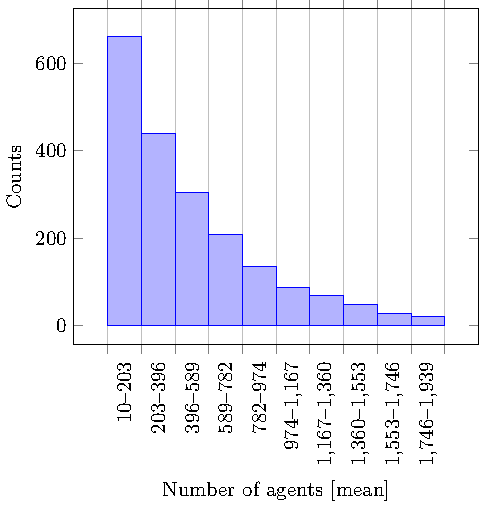
\includegraphics[height=6cm]{./appendix/trafficInfluence/Figure13}%
\caption[Parameter number of agents: histogram]{Parameter number of agents: histogram. I generate it from a negative exponential distribution. I draw many  samples where $n$ is small to detect the effect of shadowing. Figure from my publication~\cite{mayr-2021-com}.}
\label{fig:histNum}%
\end{figure}%

The second parameter is the radio transmitter power $p$ which affects how far
agents can communicate. If the power is low, messages only reach agents that are
close by. Information dissemination over large distances fails (\lq
range-problem\rq). The reception in the deployed model is based on the
signal to interference plus noise (SINR) ratio. If the SINR of a given
transmission exceeds a threshold, the transmission is correctly received. I choose a threshold of {of} 6\,dB to be on the safe side (typically 4dB are used as default). Furthermore, I assume that
the radio transmitter power is equal and constant for all mobile phones within a  sample. This is a
simplification since in reality, $p$ depends on the
local situation and the device itself. I vary the transmitter power in the range 0.5\,\dots\,2.0\,mW Equivalent Isotropically Radiated Power (EIRP).

The third parameter is the network load caused by other apps. While traveling people listen to music, use navigation apps, check their emails.  Some even watch movies while walking. To make the simulation more realistic, I assume that agents use apps which produce load in the range of $ 0... 0.20$\,MB/s. This range contains listening to music ($0.01 ... 0.03$\,MB/s), using navigation apps ($0.05$\,MB/s) and even streaming videos in low-quality ($0.06$\,MB/s).
The load ${tr}$ depends on the packet inter-transmission interval $d_{tx}$ and the packet size $s_d$ \begin{equation}
{tr} = s_d \frac{1} {d_{tx}}
\label{eq:trafSize}
\end{equation}
A constant inter-transmission interval is used assuming one-packet messages. I control the packet size $s_d$ to vary the amount of load in the model. The inter-transmission interval $d_{tx}$ is defined by the (re-)broadcast interval, which is fixed to $20$\,ms. The corresponding packet size $s_d$ is between $0 ... 4000$\,B. I expect that the information dissemination might be disturbed if the network load is high.


\begin{table}[H]
\begin{footnotesize}
\begin{tabular}{@{}llrrl@{}}%
\toprule
Parameter                        & Unit & Lower bound & Upper bound & Distribution                                    type \\ \midrule
Number of agents $n$ & 1    & 10          & 2000      & Truncated exponential (Eq.~\ref{eq:expon})  \\
Transmitter power $p$      & mW   & 0.5         & 2.0       & Uniform   \\
Packet size $s_d$        & B    & 0           & 4000        & Uniform  \\
\bottomrule 
\end{tabular}%
\end{footnotesize}
\begin{footnotesize}

\bigskip
\noindent

\begin{tabular}{@{}llllll@{}}
\toprule
Dependent parameter & Equation & Unit & Lower Bound & Upper bound & Distribution \\ \midrule
Network load ${tr}$    & see Eq.~\ref{eq:trafSize}           & MB/s    & 0          & 0.20      & Uniform                                             \\ \bottomrule
\end{tabular}
\end{footnotesize}
\caption[Uncertain parameters in the network traffic study]{Uncertain parameters in the network traffic study. I want to to know how three uncertain parameters affect the dissemination time $t_{diss}$. The packet size $s_d$ controls the amount of network load ${tr}$.}%
\label{tab:parameter}%
\end{table}%

I run $20$ simulations in parallel on a server with $80$ i7 Intel cores and $250$\,GB RAM. The simulation of $2000$ samples takes more than $6$ days including two restarts of the script that manages the simulations in parallel.

\subsection*{Effect of shadowing and network load}%
\label{sec:simulationResults}

Fig.~\ref{fig:scatter} (left) depicts that information is disseminated quickly ($t_{diss}<10s$) when the number of agents exceeds $n\approx500$. The higher the network traffic that is indicated by the message size, the longer it takes to disseminate information, see Fig.~\ref{fig:scatter} (right). Fig.~\ref{fig:subresults} shows the combined effect of shadowing with network load. When shadowing occurs, agents communicate irregularly and only for short periods. If network load is present during these periods, the information spread can be impeded. The effect seems to vanish, if the number of agents is large enough, and communication is possible at any time. 


\begin{figure}[hbt!]
\centering
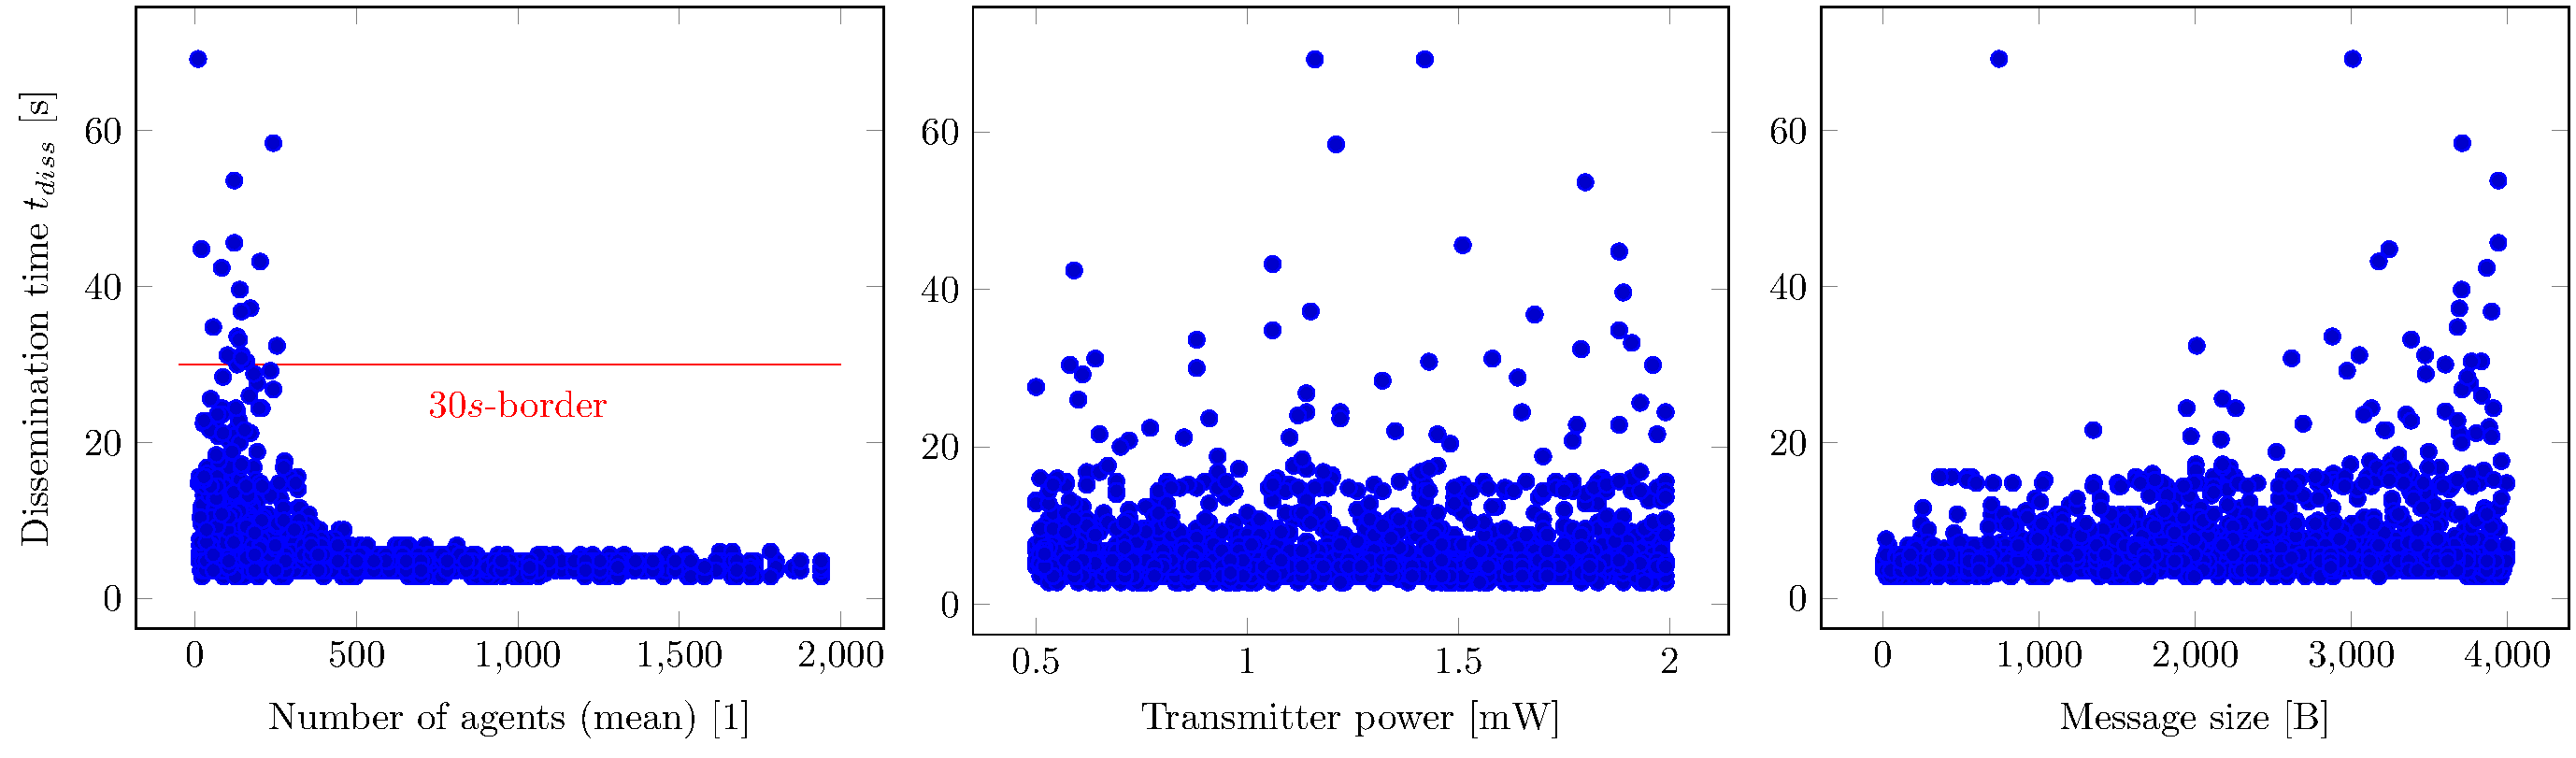
\includegraphics[width=\textwidth]{./appendix/trafficInfluence/Figure14}%
\caption[Dissemination time over the three parameters]{Dissemination time $t_{diss}$ in dependency of the number of agents (left), the transmitter power (middle), and the packet size (right) that is proportional to the network load. Only $1.1$\,\% of the data points exceed the $30$\,s-border. Note: The sample values of the two remaining parameters have been projected in the plane. Figure taken from my publication~\cite{mayr-2021-com}. }%
\label{fig:scatter}%
\end{figure}

\begin{figure}[H]
\centering
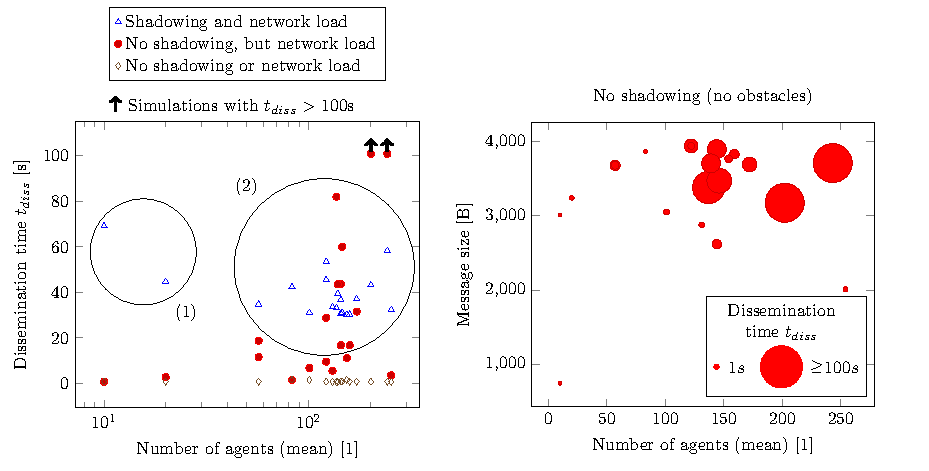
\includegraphics[width=14cm]{./appendix/trafficInfluence/Figure22}%
\caption[Simulations with delayed information dissemination times]{Simulations with delayed information dissemination times. Network load can lead to high dissemination times. Figure taken from my publication~\cite{mayr-2021-com}.}%
\label{fig:subresults}%
\end{figure}%









\chapter{Capacity estimation (Section 4.2)}
\label{sec:capacityestimation}
To estimate the minimum compliance necessary to avoid congestion in Section~\ref{sec:umleitalgorithmen}, I employ the jamming criterion that requires the capacity of bottleneck. The capacity can be either measured using a fundamental diagram or taken from handbooks. 
Fig. depicts the fundamental diagram of the scenario presented in Section~\ref{sec:umleitalgorithmen}. The densities and velocities were measured in the short route. The specific flow $J_S$ was computed using the relationship between density $d$ and velocity $v$ $J_S=d v $. One observes that the maximum flow is $J_C=1.58 ped/(ms)$, see Fig.~\ref{fig:capaestimateion}.
This value is higher than values from handbooks: Weidmann~\cite{weidmann-1994-cdyn} proposes a value of $1.23 ped/(ms)$, Fruin \cite{fruin-1964-cdyn} proposes $1.43 ped/(ms)$, while the SFPE handbook~\cite{hurley-2016-cdyn} provides a value of $1.30 ped/(ms)$. I think that this peak value is an overestimation of the actual flow caused by the small measurement interval of 0.4s. The average value computed with a polynomial regression model is much lower with $J_C=1.30 ped/(ms)$ which is in line with the handbook values. Therefore, I use a capacity of $J_C=1.30 ped/(ms)$ in my flow estimations.



\begin{figure}[hbt!]
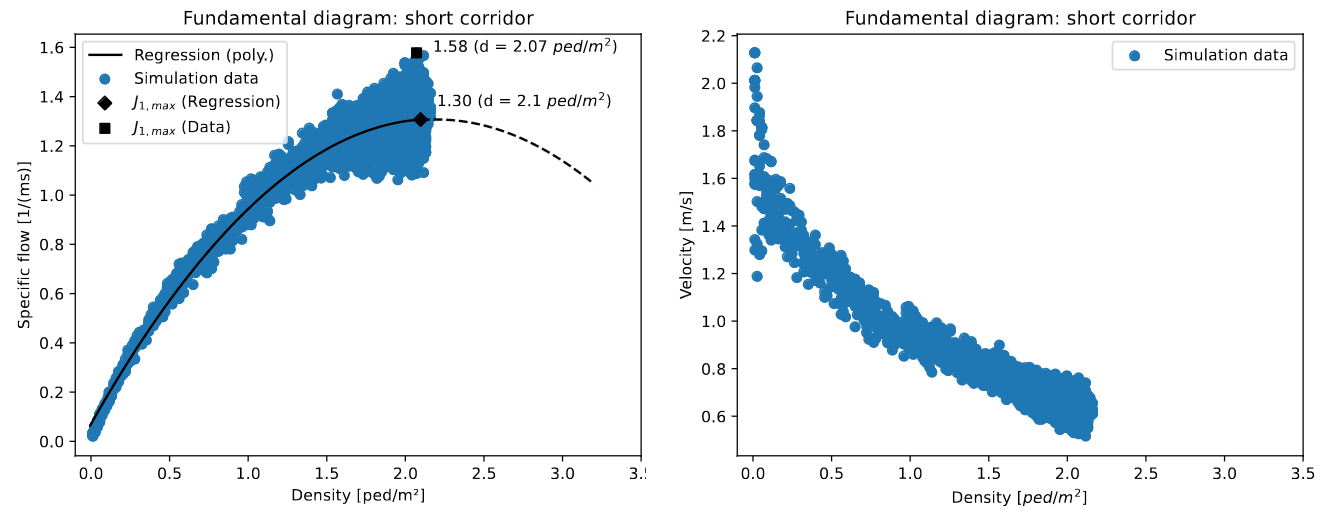
\includegraphics[width=\textwidth]{../figures/appendix/capacityestimation.png} 
\caption[Fundamental diagrams for the short route]{Fundamental diagrams for the short route. The specific flow is $J_S=\rho v $. The maximum flow is $J_C=1.58 ped/(ms)$. Image as in the publication~\cite{mayr-2022-cdyn}}
\label{fig:capaestimateion}
\end{figure}


 



\chapter{Online survey: ethical approval (Section 4.3)}
\label{sec:ethicalapproval}

Ethical approval for the online survey was obtained by the Ethics Committee of Hochschule München University of Applied Sciences (Germany, Munich). The approval comprising the conduction of the survey and the publishing of results. It was approved on 10 August 2021.


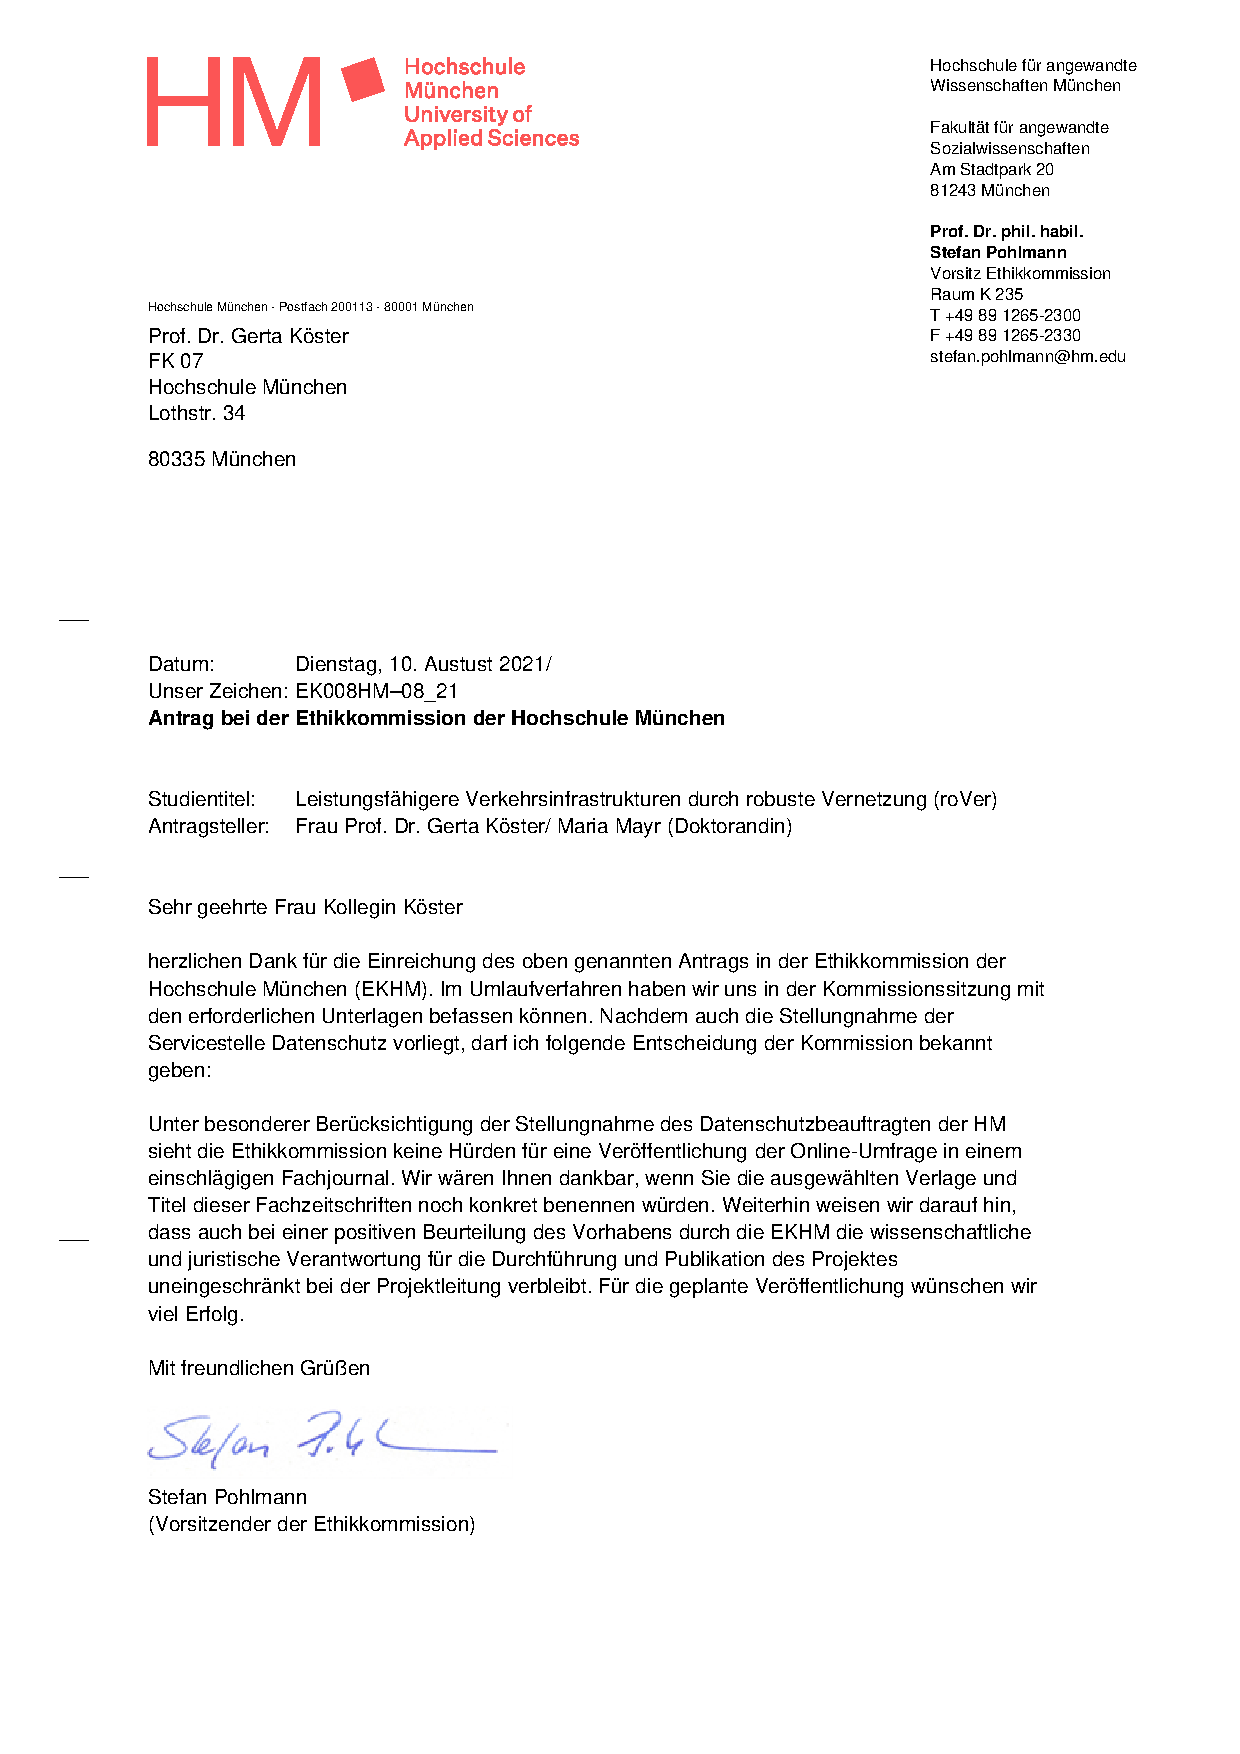
\includepdf[]{./appendix/Approval.pdf}



\chapter{Online survey: collection of statistical tests (Section 4.3)}
\label{sec:collectiontables}
The following tables contain data from statistical tests and mean values that I refer to in Section~\ref{sec:reaction}. I have published the tables as supplementary material together with my publication~\cite{mayr-2023-cdyn}. They are available online under \url{https://doi.org/10.1371/journal.pone.0284540.s004}.


\begin{table}[H]
\begin{tabular}{llrrrr}
\multicolumn{6}{c}{\textbf{Prior to information}}\\                                                                                                                                         
  \hline
Route & Group &\multicolumn{3}{l}{Route attractiveness}                                                                                                                                            &  \\ 
 &  &mean & median & std & sample size \\
  \hline
 Long & Fan & 2.124 & 2 & 0.989 & 921 \\ 
  Medium & Fan & 2.904 & 3 & 1.068 & 921 \\ 
  Short & Fan & 4.636 & 5 & 0.807 & 921 \\ 
 Long & Student \& faculty associate & 2.128 & 2 & 1.038 & 444 \\ 
  Medium & Student \& faculty associate  & 2.631 & 2 & 1.042 & 444 \\ 
Short & Student \& faculty associate  & 4.732 & 5 & 0.700 & 444 \\ 
   \hline
\end{tabular}
\caption[]{Route attractiveness prior to information (5-Point Likert scale). Two surveys were conducted: one with students \& and faculty associates and one with football fans.
For each route, participants were asked how likely it is that they take the respective route when no route recommendation is provided. Since no information is provided, the message design does not have any effect (see Tab.~\ref{tab:surveyS2G}).}
\label{tab:surveyS2E}
\end{table}


\begin{table}[H]
\begin{tabular}{llrrr}
  \hline
Comparison of attractiveness & Group & Z & $p$  \\ 
  \hline
Long route and Medium route & Fan &  -11.6806 & 0.0000  \\ 
Long route and Short route & Fan &  -38.0125 & 0.0000  \\ 
 Medium route and Short route &Fan &  -26.3319 & 0.0000  \\ 
  Long route and Medium route & Student \& faculty associate &  -5.4089 & 0.0000  \\ 
 Long route and Short route & Student \& faculty associate &  -26.3982 & 0.0000  \\ 
 Medium route and Short route & Student \& faculty associate &  -20.9893 & 0.0000 \\ 
   \hline
\end{tabular}
\caption{ Route preference prior to information. For each group, the route attractiveness of the short, medium and long route differ significantly (Dunn's test). In every comparison, the shorter route is preferred ($Z < 0$).
I conclude that there is a clear route preference: the short route is favored over the medium route followed by long route (see also the mean values from Tab.~\ref{tab:surveyS2E}).}
\label{tab:surveyS2F}
\end{table}


\begin{table}[H]
\centering
\begin{tabular}{lllrrr}
\multicolumn{6}{c}{\textbf{Information provided}}\\                                                                                                                                         

  \hline
Information & Route & Group & \textit{p} & $H$ & \textit{df} \\ 
  \hline
Prior to information &  Fans & Long &   4.5498 &      0.7150 &     7 \\ 
Prior to information &   Fans & Medium &    9.4997 &      0.2190  &     7 \\ 
Prior to information &   Fans & Short &   6.5020 &     0.4820 &     7 \\ 
Prior to information &   Students \& faculty associates & Long &          0.5950  & 5.5312 & 7 \\ 
Prior to information &   Students \& faculty associates & Medium &        0.8430 &  3.4222 & 7\\ 
Prior to information &   Students \& faculty associates & Short &         0.3660 &  7.6299 & 7 \\ 
  \hline 
After receiving information &      Fans & Long & 0.0022 & 22.42 &     7 \\ 
After receiving information &  Fans & Medium & 0.0000 & 33.04 &     7 \\ 
After receiving information &    Fans & Short & 0.0000 & 95.76 &     7 \\ 
After receiving information &  Students \& faculty associates & Long & 0.8010 & 3.811 &     7 \\ 
After receiving information &   Students \& faculty associates & Medium & 0.0000 & 32.38 &     7 \\ 
After receiving information &    Students \& faculty associates & Short& 0.0000 & 45.35 &     7 \\ 
\hline   
\end{tabular}
\caption{ Effect of message design on route attractiveness (Kruskal Wallis test). Prior to information (Tab.~\ref{tab:surveyS2E}), the message design has no effect ($p>0.05$). When information is provided (Tab.~\ref{tab:surveyS2H}), the message design has an effect ($p\leq0.05$) except for the attractiveness of the long route for the student \& faculty associate group.}
\label{tab:surveyS2G}
\end{table}

\begin{table}[H]
\begin{scriptsize}
\begin{tabular}{lllrrrr}
\multicolumn{6}{c}{\textbf{After receiving information}}\\                                                                                                                                           
  \hline
Route & Group & Message design & \multicolumn{3}{l}{Route attractiveness}                                                                                                                                            &  \\ 
 &  & &mean & median & std & n \\
 \hline
 Long & Fan & Arrow & 3.427 & 4 & 1.340 & 143 \\
   Long & Fan & Arrow + team spirit & 3.553 & 4 & 1.194 & 103 \\
   Long & Fan & Arrow + top down view & 3.550 & 4 & 1.270 & 111 \\
   Long & Fan & Arrow + top down view + team spirit & 3.743 & 4 & 1.259 & 136 \\
   Long & Fan & Congestion info + arrow & 3.505 & 4 & 1.298 & 103 \\
   Long & Fan & Congestion info + arrow + team spirit & 3.980 & 4 & 1.219 & 102 \\
   Long & Fan & Congestion info + arrow + top down view & 3.897 & 4 & 1.160 & 116 \\
   Long & Fan & Congestion info + arrow + top down view + team spirit & 3.879 & 4 & 1.079 & 107 \\
   Medium & Fan & Arrow & 3.266 & 4 & 1.156 & 143 \\
   Medium & Fan & Arrow + team spirit & 3.078 & 3 & 1.135 & 103 \\
   Medium & Fan & Arrow + top down view & 3.207 & 4 & 1.113 & 111 \\
   Medium & Fan & Arrow + top down view + team spirit & 3.066 & 3 & 1.206 & 136 \\
   Medium & Fan & Congestion info + arrow & 3.534 & 4 & 1.119 & 103 \\
   Medium & Fan & Congestion info + arrow + team spirit & 3.539 & 4 & 1.158 & 102 \\
   Medium & Fan & Congestion info + arrow + top down view & 3.655 & 4 & 1.039 & 116 \\
   Medium & Fan & Congestion info + arrow + top down view + team spirit & 3.542 & 4 & 1.093 & 107 \\
   Short & Fan & Arrow & 3.643 & 4 & 1.286 & 143 \\
   Short & Fan & Arrow + team spirit & 3.786 & 4 & 1.311 & 103 \\
   Short & Fan & Arrow + top down view & 3.414 & 4 & 1.254 & 111 \\
   Short & Fan & Arrow + top down view + team spirit & 3.265 & 3 & 1.312 & 136 \\
   Short & Fan & Congestion info + arrow & 2.806 & 2 & 1.329 & 103 \\
   Short & Fan & Congestion info + arrow + team spirit & 2.471 & 2 & 1.224 & 102 \\
   Short & Fan & Congestion info + arrow + top down view & 2.784 & 2 & 1.357 & 116 \\
   Short & Fan & Congestion info + arrow + top down view + team spirit & 2.757 & 2 & 1.265 & 107 \\
   Long & Student* & Arrow & 3.787 & 4 & 1.178 & 47 \\
   Long & Student* & Arrow + team spirit & 3.696 & 4 & 1.190 & 56 \\
   Long & Student* & Arrow + top down view & 3.938 & 4 & 1.158 & 65 \\
   Long & Student* & Arrow + top down view + team spirit & 3.823 & 4 & 1.048 & 62 \\
   Long & Student* & Congestion info + arrow & 3.862 & 4 & 1.146 & 58 \\
   Long & Student* & Congestion info + arrow + team spirit & 3.700 & 4 & 1.282 & 50 \\
   Long & Student* & Congestion info + arrow + top down view & 4.022 & 4 & 1.033 & 45 \\
   Long & Student* & Congestion info + arrow + top down view + team spirit & 3.885 & 4 & 1.305 & 61 \\
   Medium & Student* & Arrow & 2.872 & 2 & 1.191 & 47 \\
   Medium & Student* & Arrow + team spirit & 2.946 & 3 & 1.052 & 56 \\
   Medium & Student* & Arrow + top down view & 2.769 & 2 & 1.129 & 65 \\
   Medium & Student* & Arrow + top down view + team spirit & 2.903 & 3 & 1.197 & 62 \\
   Medium & Student* & Congestion info + arrow & 3.483 & 4 & 1.246 & 58 \\
   Medium & Student* & Congestion info + arrow + team spirit & 3.620 & 4 & 1.276 & 50 \\
   Medium & Student* & Congestion info + arrow + top down view & 3.622 & 4 & 1.134 & 45 \\
   Medium & Student* & Congestion info + arrow + top down view + team spirit & 3.246 & 4 & 1.247 & 61 \\
   Short & Student* & Arrow & 3.128 & 3 & 1.172 & 47 \\
   Short & Student* & Arrow + team spirit & 3.321 & 4 & 1.162 & 56 \\
   Short & Student* & Arrow + top down view & 3.338 & 3 & 1.314 & 65 \\
   Short & Student* & Arrow + top down view + team spirit & 3.403 & 3 & 1.221 & 62 \\
   Short & Student* & Congestion info + arrow & 2.483 & 2 & 1.047 & 58 \\
   Short & Student* & Congestion info + arrow + team spirit & 2.540 & 2 & 1.199 & 50 \\
   Short & Student* & Congestion info + arrow + top down view & 2.533 & 2 & 1.198 & 45 \\
   Short & Student* & Congestion info + arrow + top down view + team spirit & 2.689 & 2 & 1.218 & 61 \\
   \hline
\end{tabular}
\end{scriptsize}
\caption{Route attractiveness when recommending the long route (5-Point Likert scale). Two surveys were conducted: one with students \&  faculty associates (student*) and one with football fans.
For each route, participants were asked how likely it is that they take the respective route when a route recommendation is provided. The message design always has an effect on the attractiveness of the routes except for the attractiveness of the long route, see Kruskal Wallis tests (see Tab.~\ref{tab:surveyS2G}).}
\label{tab:surveyS2H}
\end{table}




\pagestyle{empty}

\begin{sidewaystable}
\begin{scriptsize}

\hspace{-3.0cm}
\begin{tabular}{llllrr}
\multicolumn{6}{c}{\textbf{Students \& faculty associates}} \\
\hline
 Route & Added component & Message design 1 & Message design 2 & \textit{p} &  \textit{W} \\ 
  \hline
Long & Congestion info & Arrow (mean = 3.787) & Congestion info + arrow (mean = 3.862) & 0.7592 & 1317.5 \\ 
  Long & Congestion info & Arrow + top down view (mean = 3.938) & Congestion info + arrow + top down view (mean = 4.022) & 0.8557 & 1434.0 \\ 
  Long & Congestion info & Arrow + team spirit (mean = 3.696) & Congestion info + arrow + team spirit (mean = 3.700) & 0.8356 & 1368.0 \\ 
  Long & Congestion info & Arrow + top down view + team spirit (mean = 3.823) & Congestion info + arrow + top down view + team spirit (mean = 3.885) & 0.3327 & 1708.5 \\ 
  Long & Team spirit & Congestion info + arrow (mean = 3.862) & Congestion info + arrow + team spirit (mean = 3.700) & 0.6071 & 1530.0 \\ 
  Long & Team spirit & Congestion info + arrow + top down view (mean = 4.022) & Congestion info + arrow + top down view + team spirit (mean = 3.885) & 0.9810 & 1376.5 \\ 
  Long & Team spirit & Arrow (mean = 3.787) & Arrow + team spirit (mean = 3.696) & 0.6422 & 1383.5 \\ 
  Long & Team spirit & Arrow + top down view (mean = 3.938) & Arrow + top down view + team spirit (mean = 3.823) & 0.3331 & 2205.5 \\ 
  Long & Top down view & Congestion info + arrow (mean = 3.862) & Congestion info + arrow + top down view (mean = 4.022) & 0.5715 & 1224.5 \\ 
  Long & Top down view & Congestion info + arrow + team spirit (mean = 3.700) & Congestion info + arrow + top down view + team spirit (mean = 3.885) & 0.3818 & 1384.5 \\ 
  Long & Top down view & Arrow (mean = 3.787) & Arrow + top down view (mean = 3.938) & 0.4979 & 1418.5 \\ 
  Long & Top down view & Arrow + team spirit (mean = 3.696) & Arrow + top down view + team spirit (mean = 3.823) & 0.6822 & 1663.0 \\ 
  \hline
  Medium & Congestion info & Arrow (mean = 2.872) & Congestion info + arrow (mean = 3.483) & \textbf{0.0117} & 989.0 \\ 
  Medium & Congestion info & Arrow + top down view (mean = 2.769) & Congestion info + arrow + top down view (mean = 3.622) & \textbf{0.0003} & 884.5 \\ 
  Medium & Congestion info & Arrow + team spirit (mean = 2.946) & Congestion info + arrow + team spirit (mean = 3.620) & \textbf{0.0031} & 949.5 \\ 
  Medium & Congestion info & Arrow + top down view + team spirit (mean = 2.903) & Congestion info + arrow + top down view + team spirit (mean = 3.246) & 0.1243 & 1598.5 \\ 
  Medium & Team spirit & Congestion info + arrow (mean = 3.483) & Congestion info + arrow + team spirit (mean = 3.62) & 0.4871 & 1341.0 \\ 
  Medium & Team spirit & Congestion info + arrow + top down view (mean = 3.622) & Congestion info + arrow + top down view + team spirit (mean = 3.246) & 0.1283 & 1601.5 \\ 
  Medium & Team spirit & Arrow (mean = 2.872) & Arrow + team spirit (mean = 2.946) & 0.6933 & 1259.5 \\ 
  Medium & Team spirit & Arrow + top down view (mean = 2.769) & Arrow + top down view + team spirit (mean = 2.903) & 0.5484 & 1895.5 \\ 
  Medium & Top down view & Congestion info + arrow (mean = 3.483) & Congestion info + arrow + top down view (mean = 3.622) & 0.6519 & 1240.0 \\ 
  Medium & Top down view & Congestion info + arrow + team spirit (mean = 3.62) & Congestion info + arrow + top down view + team spirit (mean = 3.246) & 0.1017 & 1792.5 \\ 
  Medium & Top down view & Arrow (mean = 2.872) & Arrow + top down view (mean = 2.769) & 0.6865 & 1593.0 \\ 
  Medium & Top down view & Arrow + team spirit (mean = 2.946) & Arrow + top down view + team spirit (mean = 2.903) & 0.7897 & 1783.5 \\ 
  \hline
  Short & Congestion info & Arrow (mean = 3.128) & Congestion info + arrow (mean = 2.483) & \textbf{0.0019} & 1804.0 \\ 
  Short & Congestion info & Arrow + top down view (mean = 3.338) & Congestion info + arrow + top down view (mean = 2.533) & \textbf{0.0009} & 1974.5 \\ 
  Short & Congestion info & Arrow + team spirit (mean = 3.321) & Congestion info + arrow + team spirit (mean = 2.54) & \textbf{0.0010} & 1895.5 \\ 
  Short & Congestion info & Arrow + top down view + team spirit (mean = 3.403) & Congestion info + arrow + top down view + team spirit (mean = 2.689) & \textbf{0.0011} & 2514.5 \\ 
  Short & Team spirit & Congestion info + arrow (mean = 2.483) & Congestion info + arrow + team spirit (mean = 2.54) & 0.9363 & 1438.0 \\ 
  Short & Team spirit & Congestion info + arrow + top down view (mean = 2.533) & Congestion info + arrow + top down view + team spirit (mean = 2.689) & 0.4671 & 1270.0 \\ 
  Short & Team spirit & Arrow (mean = 3.128) & Arrow + team spirit (mean = 3.321) & 0.4109 & 1196.5 \\ 
  Short & Team spirit & Arrow + top down view (mean = 3.338) & Arrow + top down view + team spirit (mean = 3.403) & 0.7408 & 1948.0 \\ 
  Short & Top down view & Congestion info + arrow (mean = 2.483) & Congestion info + arrow + top down view (mean = 2.533) & 0.9657 & 1311.0 \\ 
  Short & Top down view & Congestion info + arrow + team spirit (mean = 2.54) & Congestion info + arrow + top down view + team spirit (mean = 2.689) & 0.5119 & 1422.5 \\ 
  Short & Top down view & Arrow (mean = 3.128) & Arrow + top down view (mean = 3.338) & 0.4113 & 1393.0 \\ 
  Short & Top down view & Arrow + team spirit (mean = 3.321) & Arrow + top down view + team spirit (mean = 3.403) & 0.6679 & 1658.5 \\ 
\hline
\end{tabular}

\end{scriptsize}

\caption[]{Effect of message component on how \textbf{students \& faculty associates} evaluate the route attractiveness (Mann Whitney U test). If adding a component makes a significant difference ($p<0.05$) the corresponding \textit{p}-Value is marked bold. The mean values '(mean = ...)` represent the respective mean values of the route attractivenesses (see Tab.~\ref{tab:surveyS2H} for the full statistics of the route attractivenesses).}
\label{tab:surveyS2A}
\end{sidewaystable}


\begin{sidewaystable}
\begin{scriptsize}
\hspace{-3.0cm}
\begin{tabular}{llllrr}
\multicolumn{6}{c}{\textbf{Fans}} \\
\hline
 Route & Added component & Message design 1 & Message design 2 & \textit{p} &  \textit{W} \\ 
  \hline
Long & Congestion info & Arrow (mean = 3.427) & Congestion info + arrow (mean = 3.505) & 0.6181 & 7099.5 \\
  Long & Congestion info & Arrow + top down view (mean = 3.55) & Congestion info + arrow + top down view (mean = 3.897) & \textbf{0.0331} & 5433.0 \\
  Long & Congestion info & Arrow + team spirit (mean = 3.553) & Congestion info + arrow + team spirit (mean = 3.980) & \textbf{0.0047} & 4107.0 \\
  Long & Congestion info & Arrow + top down view + team spirit (mean = 3.743) & Congestion info + arrow + top down view + team spirit (mean = 3.879) & 0.6983 & 7076.0 \\
  Long & Team spirit & Congestion info + arrow (mean = 3.505) & Congestion info + arrow + team spirit (mean = 3.980) & \textbf{0.0069} & 4157.0 \\
  Long & Team spirit & Congestion info + arrow + top down view (mean = 3.897) & Congestion info + arrow + top down view + team spirit (mean = 3.879) & 0.6011 & 6443.0 \\
  Long & Team spirit & Arrow (mean = 3.427) & Arrow + team spirit (mean = 3.553) & 0.5517 & 7048.5 \\
  Long & Team spirit & Arrow + top down view (mean = 3.55) & Arrow + top down view + team spirit (mean = 3.743) & 0.1957 & 6856.0 \\
  Long & Top down view & Congestion info + arrow (mean = 3.505) & Congestion info + arrow + top down view (mean = 3.897) & \textbf{0.0305} & 5006.0 \\
  Long & Top down view & Congestion info + arrow + team spirit (mean = 3.980) & Congestion info + arrow + top down view + team spirit (mean = 3.879) & 0.1645 & 6028.0 \\
  Long & Top down view & Arrow (mean = 3.427) & Arrow + top down view (mean = 3.55) & 0.5125 & 7570.5 \\
  Long & Top down view & Arrow + team spirit (mean = 3.553) & Arrow + top down view + team spirit (mean = 3.743) & 0.1652 & 6299.0 \\
    \hline
  Medium & Congestion info & Arrow (mean = 3.266) & Congestion info + arrow (mean = 3.534) & 0.0731 & 6423.5 \\
  Medium & Congestion info & Arrow + top down view (mean = 3.207) & Congestion info + arrow + top down view (mean = 3.655) & \textbf{0.0021} & 5006.5 \\
  Medium & Congestion info & Arrow + team spirit (mean = 3.078) & Congestion info + arrow + team spirit (mean = 3.539) & \textbf{0.0038} & 4087.5 \\
  Medium & Congestion info & Arrow + top down view + team spirit (mean = 3.066) & Congestion info + arrow + top down view + team spirit (mean = 3.542) & \textbf{0.0022} & 5678.0 \\
  Medium & Team spirit & Congestion info + arrow (mean = 3.534) & Congestion info + arrow + team spirit (mean = 3.539) & 0.8731 & 5188.5 \\
  Medium & Team spirit & Congestion info + arrow + top down view (mean = 3.655) & Congestion info + arrow + top down view + team spirit (mean = 3.542) & 0.4670 & 6535.0 \\
  Medium & Team spirit & Arrow (mean = 3.266) & Arrow + team spirit (mean = 3.078) & 0.1820 & 8065.5 \\
  Medium & Team spirit & Arrow + top down view (mean = 3.207) & Arrow + top down view + team spirit (mean = 3.066) & 0.3322 & 8066.0 \\
  Medium & Top down view & Congestion info + arrow (mean = 3.534) & Congestion info + arrow + top down view (mean = 3.655) & 0.4556 & 5644.5 \\
  Medium & Top down view & Congestion info + arrow + team spirit (mean = 3.539) & Congestion info + arrow + top down view + team spirit (mean = 3.542) & 0.9011 & 5508.5 \\
  Medium & Top down view & Arrow (mean = 3.266) & Arrow + top down view (mean = 3.207) & 0.6396 & 8195.5 \\
  Medium & Top down view & Arrow + team spirit (mean = 3.078) & Arrow + top down view + team spirit (mean = 3.066) & 0.9352 & 7045.5 \\
  \hline
  Short & Congestion info & Arrow (mean = 3.643) & Congestion info + arrow (mean = 2.806) & \textbf{0.0000} & 9855.0 \\
  Short & Congestion info & Arrow + top down view (mean = 3.414) & Congestion info + arrow + top down view (mean = 2.784) & \textbf{0.0003} & 8143.0 \\
  Short & Congestion info & Arrow + team spirit (mean = 3.786) & Congestion info + arrow + team spirit (mean = 2.471) & \textbf{0.0000} & 7940.5 \\
  Short & Congestion info & Arrow + top down view + team spirit (mean = 3.265) & Congestion info + arrow + top down view + team spirit (mean = 2.757) & \textbf{0.0023} & 8857.5 \\
  Short & Team spirit & Congestion info + arrow (mean = 2.806) & Congestion info + arrow + team spirit (mean = 2.471) & 0.0634 & 5993.5 \\
  Short & Team spirit & Congestion info + arrow + top down view (mean = 2.784) & Congestion info + arrow + top down view + team spirit (mean = 2.757) & 0.9759 & 6192.0 \\
  Short & Team spirit & Arrow (mean = 3.643) & Arrow + team spirit (mean = 3.786) & 0.3306 & 6851.5 \\
  Short & Team spirit & Arrow + top down view (mean = 3.414) & Arrow + top down view + team spirit (mean = 3.265) & 0.3873 & 8015.0 \\
  Short & Top down view & Congestion info + arrow (mean = 2.806) & Congestion info + arrow + top down view (mean = 2.784) & 0.8446 & 6060.5 \\
  Short & Top down view & Congestion info + arrow + team spirit (mean = 2.471) & Congestion info + arrow + top down view + team spirit (mean = 2.757) & 0.0781 & 4740.5 \\
  Short & Top down view & Arrow (mean = 3.643) & Arrow + top down view (mean = 3.414) & 0.1237 & 8799.5 \\
  Short & Top down view & Arrow + team spirit (mean = 3.786) & Arrow + top down view + team spirit (mean = 3.265) & \textbf{0.0024} & 8555.5 \\
   \hline
\end{tabular}
\end{scriptsize}
\caption[]{Effect of message component on how \textbf{fans} evaluate the route attractiveness (Mann Whitney U test). If adding a component makes a significant difference ($p<0.05$) the corresponding p-Value is marked bold. The mean values '(mean = ...)` represent the respective mean values of the route attractivenesses (see Tab.~\ref{tab:surveyS2H} for the full statistics of the route attractiveness)}
\label{tab:surveyS2B}
\end{sidewaystable}


\clearpage


%Kopf- und Fußzeile
\pagestyle{fancy}
\fancyhf{}
 
%Kopfzeile mittig mit Kaptilname
%\fancyhead[C]{\textsf{\nouppercase{\leftmark}}}

\fancyhead[C]{\textsf{ {\thechapter} \nouppercase{\leftmark} }}


%\fancyhead[R]{ \includegraphics[height=1.2cm]{./pictures/hm_logo_alt} } %\input{./pictures/image.pdf_tex}  }
%Linie oben
%\renewcommand{\headrulewidth}{0.5pt}
%Fußzeile links bzw. innen
	%\fancyfoot[L]{Christina Maria Mayr}
	\fancyfoot[C]{\thepage}
%Linie unten
%\renewcommand{\footrulewidth}{0.5pt}
 
% Fußzeile auf jeder Seite - auch Kapitel und Inhaltsverzeichnis
\fancypagestyle{plain}{%
   \fancyhf{}%
	%\fancyfoot[L]{Christina Maria Mayr}
	\fancyfoot[C]{\thepage}
   \renewcommand{\headrulewidth}{0.0pt} %obere Linie ausblenden
}




\addtolength{\headheight}{\baselineskip}
\addtolength{\headheight}{0.61pt}
\addtolength{\footskip}{10pt}
\renewcommand{\headrulewidth}{0pt}% Trennlinie

\renewcommand{\chaptermark}[1]{\markboth{#1}{}}


\begin{table}
\begin{scriptsize}

\begin{tabular}{llrrcc}
\multicolumn{6}{c}{ \textbf{Students \& faculty associates: Route attractiveness (mean value)}} \\
  \hline
 Route & Condition & Prior  & Info.  & \textit{p} & \textit{W} \\
   &  &  to info. & provided &  &  \\

  \hline
 Long & Arrow + top down view & 2.062 & 3.938 & \textbf{0.0000} & 3654.5 \\ 
   Long & Arrow + team spirit & 2.196 & 3.696 & \textbf{0.0000} & 2542.5 \\ 
   Long & Congestion info + arrow & 2.241 & 3.862 & \textbf{0.0000} & 2758.0 \\ 
   Long & Arrow + top down view + team spirit & 2.145 & 3.823 & \textbf{0.0000} & 3245.5 \\ 
   Long & Arrow & 2.149 & 3.787 & \textbf{0.0000} & 1834.0 \\ 
   Long & Congestion info + arrow + top down view + team spirit & 2.016 & 3.885 & \textbf{0.0000} & 3133.5 \\ 
   Long & Congestion info + arrow + top down view & 2.311 & 4.022 & \textbf{0.0000} & 1720.5 \\ 
   Long & Congestion info + arrow + team spirit & 1.940 & 3.700 & \textbf{0.0000} & 2105.0 \\ 
   \hline
   Medium & Arrow + top down view & 2.708 & 2.769 & 0.7852 & 2168.0 \\ 
   Medium & Arrow + team spirit & 2.643 & 2.946 & 0.1015 & 1825.5 \\ 
   Medium & Congestion info + arrow & 2.672 & 3.483 & \textbf{0.0004} & 2298.5 \\ 
   Medium & Arrow + top down view + team spirit & 2.677 & 2.903 & 0.2906 & 2122.0 \\ 
   Medium & Arrow & 2.723 & 2.872 & 0.5057 & 1185.5 \\ 
   Medium & Congestion info + arrow + top down view + team spirit & 2.607 & 3.246 & \textbf{0.0045} & 2391.0 \\ 
   Medium & Congestion info + arrow + top down view & 2.600 & 3.622 & \textbf{0.0000} & 1503.5 \\ 
   Medium & Congestion info + arrow + team spirit & 2.380 & 3.620 & \textbf{0.0000} & 1924.0 \\ 
   \hline
   Short & Arrow + top down view & 4.754 & 3.338 & \textbf{0.0000} & 847.0 \\ 
   Short & Arrow + team spirit & 4.732 & 3.321 & \textbf{0.0000} & 465.0 \\ 
   Short & Congestion info + arrow & 4.603 & 2.483 & \textbf{0.0000} & 284.0 \\ 
   Short & Arrow + top down view + team spirit & 4.806 & 3.403 & \textbf{0.0000} & 644.0 \\ 
   Short & Arrow & 4.681 & 3.128 & \textbf{0.0000} & 342.0 \\ 
   Short & Congestion info + arrow + top down view + team spirit & 4.787 & 2.689 & \textbf{0.0000} & 357.5 \\ 
   Short & Congestion info + arrow + top down view & 4.667 & 2.533 & \textbf{0.0000} & 223.0 \\ 
   Short & Congestion info + arrow + team spirit & 4.800 & 2.540 & \textbf{0.0000} & 204.0 \\ 
   \hline
\end{tabular}
\end{scriptsize}
\caption{Effect of information provision on how \textbf{students \& faculty associates} evaluate the route attractiveness (Mann Whitney U test). If information provision makes a significant difference ($p<0.05$) the corresponding \textit{p}-Value is marked bold. Through information the long route becomes always more attractive (the means increase), while the short route always becomes less attractive (the means reduce). Also, the medium route becomes more attractive. The increase of the means is not always significant.}
\label{tab:surveyS2C}
\end{table}



\begin{table}
\begin{scriptsize}
\begin{tabular}{llrrrr}
\multicolumn{6}{c}{ \textbf{Fans: Route attractiveness (mean value)}} \\
  \hline
 Route & Condition & Prior  & Info.  & \textit{p} & \textit{W} \\
   &  &  to info. & provided &  &  \\
  \hline
 Long & Arrow + top down view & 2.207 & 3.550 & \textbf{0.0000} & 9524.0 \\ 
 Long & Arrow + team spirit & 2.146 & 3.553 & \textbf{0.0000} & 8471.5 \\ 
 Long & Congestion info + arrow & 1.981 & 3.505 & \textbf{0.0000} & 8584.5 \\ 
 Long & Arrow + top down view + team spirit & 2.125 & 3.743 & \textbf{0.0000} & 15171.0 \\ 
 Long & Arrow & 2.035 & 3.427 & \textbf{0.0000} & 15846.0 \\ 
 Long & Congestion info + arrow + top down view + team spirit & 2.131 & 3.879 & \textbf{0.0000} & 9755.0 \\ 
 Long & Congestion info + arrow + top down view & 2.259 & 3.897 & \textbf{0.0000} & 11034.0 \\ 
 Long & Congestion info + arrow + team spirit & 2.118 & 3.980 & \textbf{0.0000} & 8914.0 \\ 
 \hline
 Medium & Arrow + top down view & 2.793 & 3.207 & \textbf{0.0053} & 7424.5 \\ 
 Medium & Arrow + team spirit & 2.816 & 3.078 & 0.0991 & 5969.0 \\ 
 Medium & Congestion info + arrow & 2.718 & 3.534 & \textbf{0.0000} & 7383.0 \\ 
 Medium & Arrow + top down view + team spirit & 3.029 & 3.066 & 0.8674 & 9352.0 \\ 
 Medium & Arrow & 2.909 & 3.266 & \textbf{0.0045} & 12116.5 \\ 
 Medium & Congestion info + arrow + top down view + team spirit & 3.028 & 3.542 & \textbf{0.0005} & 7214.5 \\ 
 Medium & Congestion info + arrow + top down view & 2.974 & 3.655 & \textbf{0.0000} & 8926.5 \\ 
 Medium & Congestion info + arrow + team spirit & 2.922 & 3.539 & \textbf{0.0001} & 6799.5 \\ 
 \hline
 Short & Arrow + top down view & 4.523 & 3.414 & \textbf{0.0000} & 2913.5 \\ 
 Short & Arrow + team spirit & 4.670 & 3.786 & \textbf{0.0000} & 3165.0 \\ 
 Short & Congestion info + arrow & 4.583 & 2.806 & \textbf{0.0000} & 1690.5 \\ 
 Short & Arrow + top down view + team spirit & 4.669 & 3.265 & \textbf{0.0000} & 3666.5 \\ 
 Short & Arrow & 4.692 & 3.643 & \textbf{0.0000} & 5235.0 \\ 
 Short & Congestion info + arrow + top down view + team spirit & 4.654 & 2.757 & \textbf{0.0000} & 1507.5 \\ 
 Short & Congestion info + arrow + top down view & 4.560 & 2.784 & \textbf{0.0000} & 2294.0 \\ 
 Short & Congestion info + arrow + team spirit & 4.725 & 2.471 & \textbf{0.0000} & 935.5 \\ 
   \hline
\end{tabular}
\end{scriptsize}
\caption{Effect of information provision on how \textbf{football fans} evaluate the route attractiveness (Mann Whitney U test). If information provision makes a significant difference ($p<0.05$) the corresponding \textit{p}-Value is marked bold. Through information the long route becomes always more attractive (the means increase), while the short route always becomes less attractive (the means reduce). Also, the medium route becomes more attractive. The increase of the means is not always significant.}
\label{tab:surveyS2D}
\end{table}



\chapter{Familiarity with environment (Section 4.3)}
\label{sec:navigation}

Findings from the online survey strongly indicate that people are basically willing to follow instructions provided by mobile applications. However, the survey assumed that people are familiar with the environment.
To find out how well people can follow the recommendation under real environmental conditions, I am conducting an on-site survey at the metro station Münchner Freiheit (Munich, Germany).
The survey was conducted by Christina Mayr as part of the \textit{roVer} project on 26 September 2023 (14:00-15:00) at the surface level of the train station. The procedure was as follows:
\begin{itemize}
\item Approach people (say: I'm from Munich University of Applied Sciences and I'm conducting a scientific survey together with MVG. One question for you - it will only take 10 seconds.)
\item Then show the picture (see fig.~\ref{fig:msg}) on a tablet and ask: "How well can you find the way. Please rate with a school grade."
\item Note the school grade.
\end{itemize}
18 people took part in the survey. 17 out of 18 people provided an answer. 11 out of 17 people provided information on their local knowledge without being asked.

\begin{figure}[hbt!]
\centering
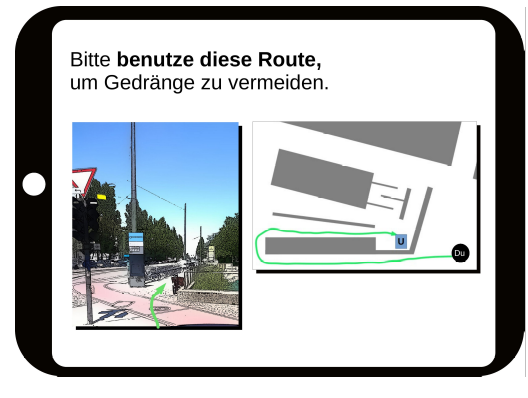
\includegraphics[width=8cm]{../figures/appendix/onsite.png} 
\caption[Message design]{Message design}
\label{fig:msg}
\end{figure}


The survey indicates that people familiar with the area can easily find the recommended route, see Fig.~\ref{fig:familair}. All 6 people with local knowledge gave the school grade "very good" (1). People who are not familiar with the area have problems finding the route (rating: 4 or 5). However, 2 out of 5 people found the non-recommended direct route thanks to the signposting on site. These two people also stated that they would find it helpful if the suggested route was signposted. No tendency can be observed for people who did not indicate their local knowledge. 2 out of 6 people found it easy to find the route ("very good"). 2 out of 6 people think that finding the route is challenging ("satisfactory"). 2 out of 6 people find it difficult (grade 4 or 6).

The survey sample was small and is not representative. For a representative study, a much larger number of survey participants would be necessary, as well as the recording of other factors such as day of the week, time of day, age distribution, etc. 
Nevertheless, a tendency can already be identified from this small sample. People who are familiar with the area seem to have no problems finding the recommended route. People who are not familiar with the area may have problems finding their way. 
One way to make orientation on the surface of Münchner Freiheit generally easier would be to signpost alternative routes with the aid of static signs. If an app were to be developed, orientation could be supported, for example, with a live view such as Google Maps Live View.




\begin{figure}[hbt!]
\centering
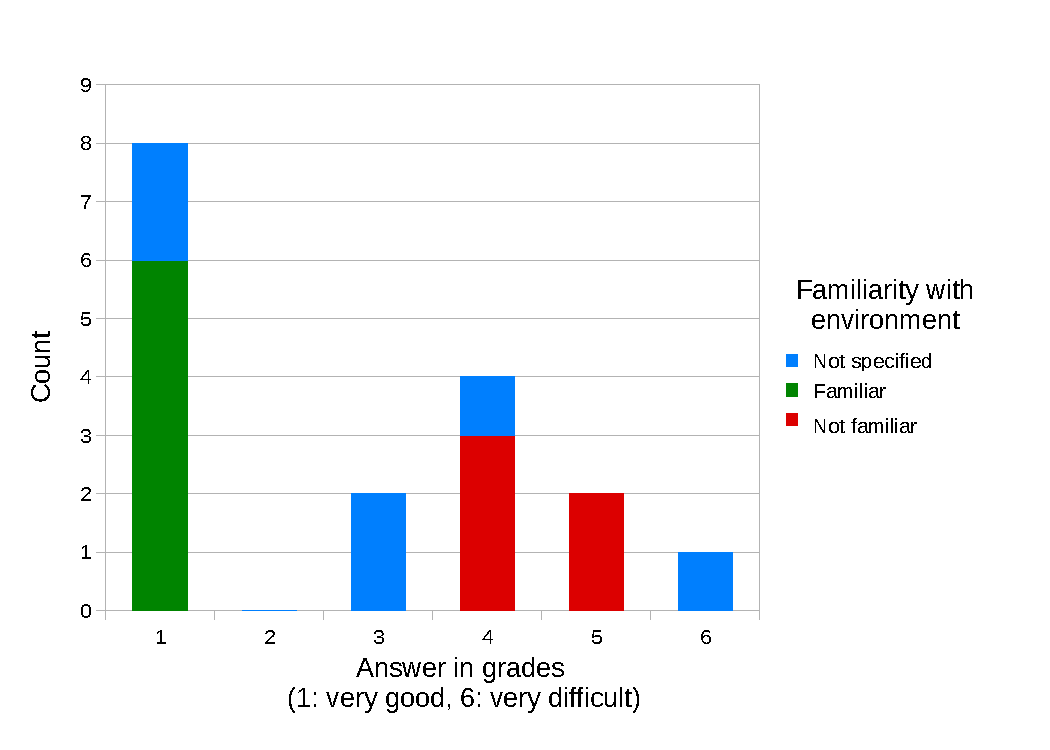
\includegraphics[width=12cm]{../figures/appendix/resultsonsite.pdf} 
\caption[Effect of familiarity on navigation]{Effect of familiarity on navigation. }
\label{fig:familair}
\end{figure}





\chapter{Pedestrian streams at Münchner Freiheit (Section 4.4)}
\label{sec:countstudy}

On 29th Oct 2020 I conducted a counting study at the metro station Münchner Freiheit (Munich, Germany). The results of the counting study will be published soon in the conference proceedings \textit{Collective Dynamics}: The title is \textit{Estimating pedestrian flows using route distributions and sparse counting data}. 
To carry out the counting experiment, I had obtained permission from the local transport provider Münchner Verkehrsgesellschaft mbH (MVG) in Munich, Germany.  Fig.~\ref{fig:intermediatefloormucfreiheit} depicts a map of the intermediate floor of the metro station.  





\begin{figure}[H]
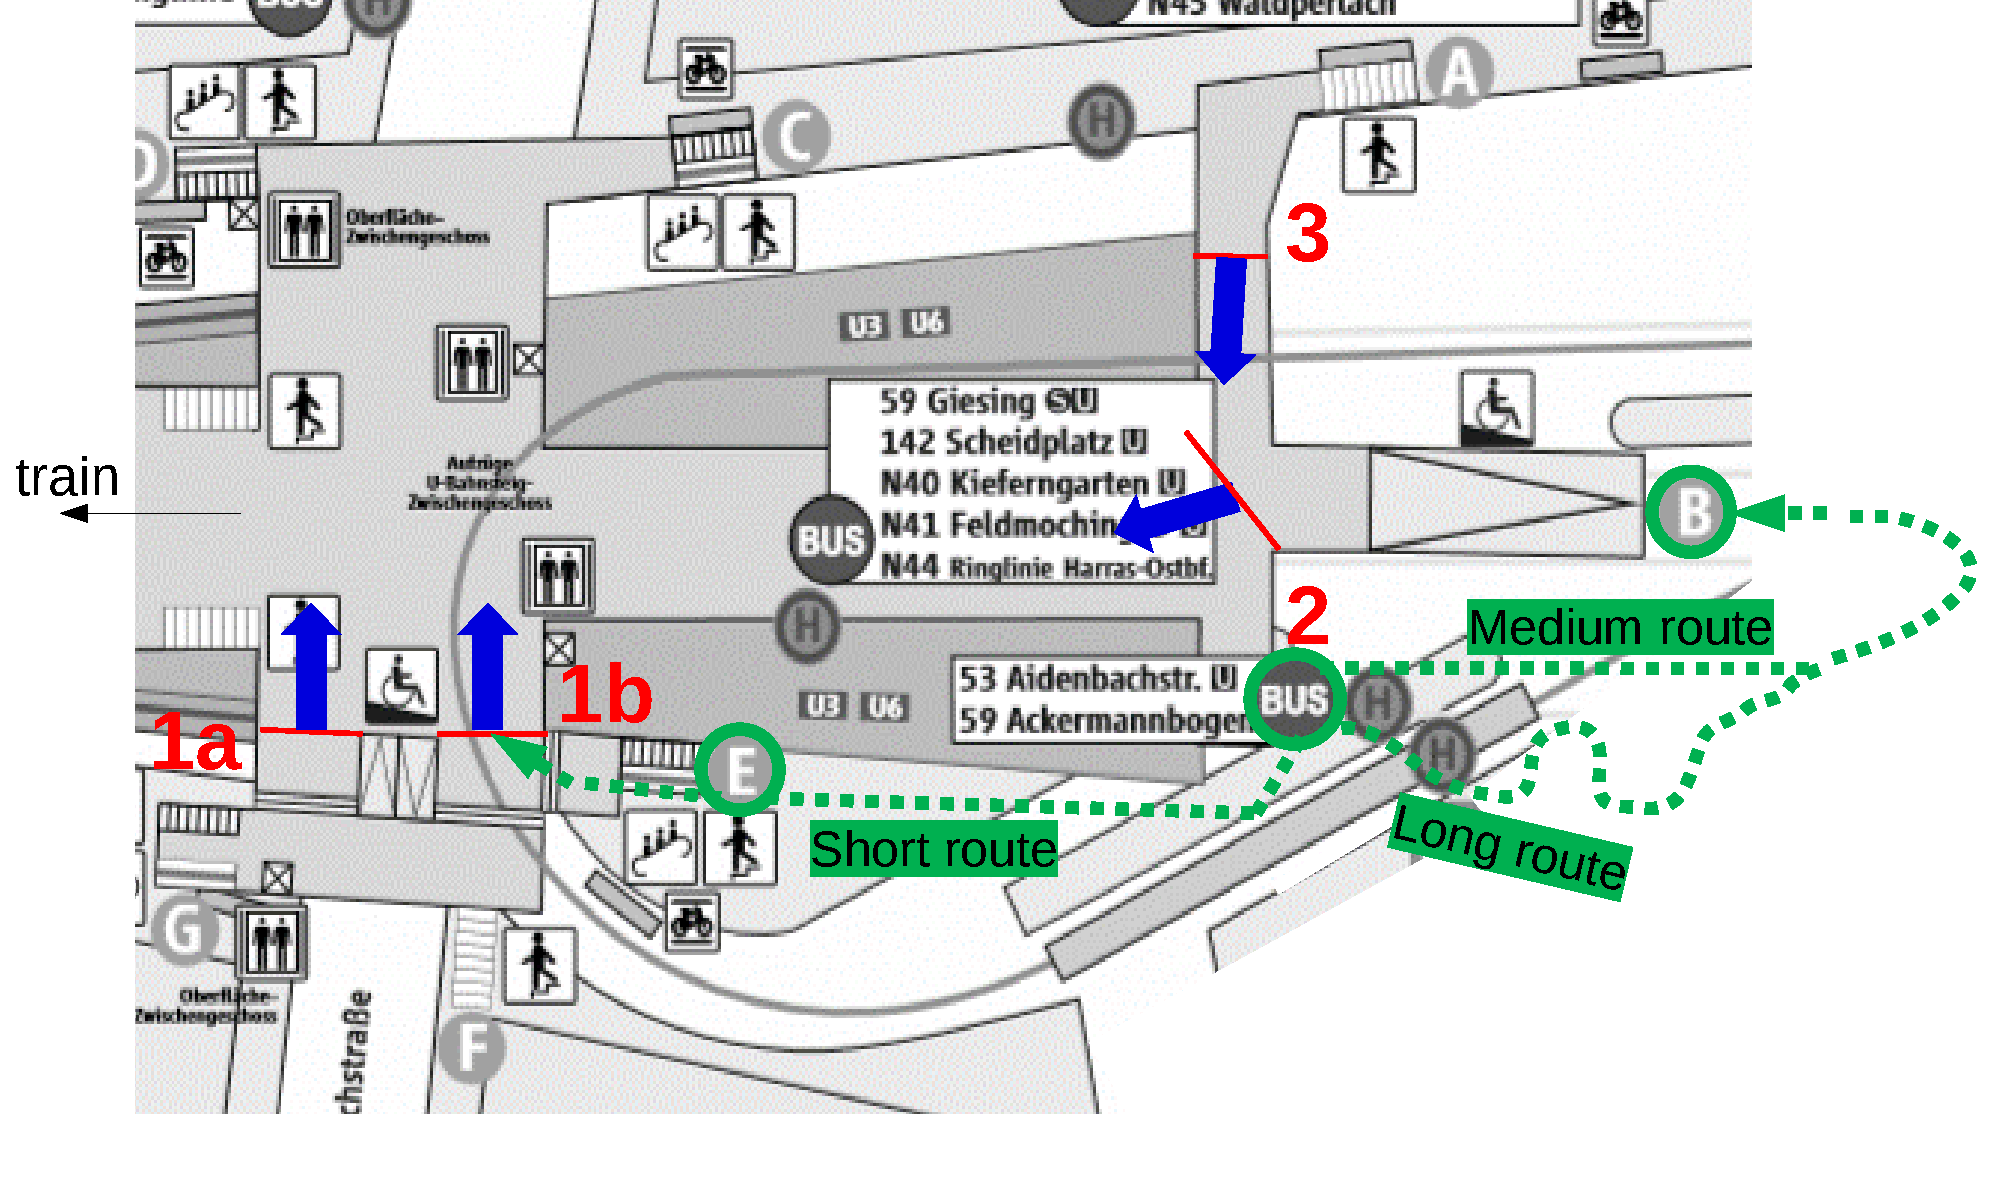
\includegraphics[width=0.7\textwidth]{./appendix/countingExperiment/MeasurementLines.pdf} 
\includegraphics[width=0.3\textwidth]{./appendix/countingExperiment/Messstellen_Fotos_1b.pdf} 
\includegraphics[width=0.3\textwidth]{./appendix/countingExperiment/Messstellen_Fotos_2.pdf} 
\includegraphics[width=0.3\textwidth]{./appendix/countingExperiment/Messstellen_Fotos_3.pdf} 
\caption[Counting experiment: location of the measurement lines.]{Counting experiment: location of the measurement lines. Students clicked an app whenever a person crossed an imaginary line towards a certain direction. The map in the background (top) was taken from \url{https://efa.mvv-muenchen.de/sta/muenchnerfreiheit.pdf} (16th Jan. 2023). I added arrows and routes. Own photographs (bottom). }
\label{fig:intermediatefloormucfreiheit}
\end{figure}


Students counted pedestrians at various points on the intermediate floor of the station during the afternoon in three time slots of each 30 minutes.
Students clicked an app whenever a person crossed an imaginary line towards a certain direction.


\subsection*{Arrivals over time}


Fig.~\ref{fig:timeslots} depicts the results of the counting experiment. I would like to mention that the counting experiment took place  during a lull in the Covid pandemic. Hence, the measured flows might be lower than before or after the pandemic. The flow at the measurement line 1b is always larger than the flow at the other measurement line. Unfortunately, I do not know where the arrivals come from. The arrivals  measured at line 1b can either come from the bus or side entrances. One can observe that for the measurement line 1b, the number of arrivals varies over time. 


\begin{figure}[hbt!]
\centering
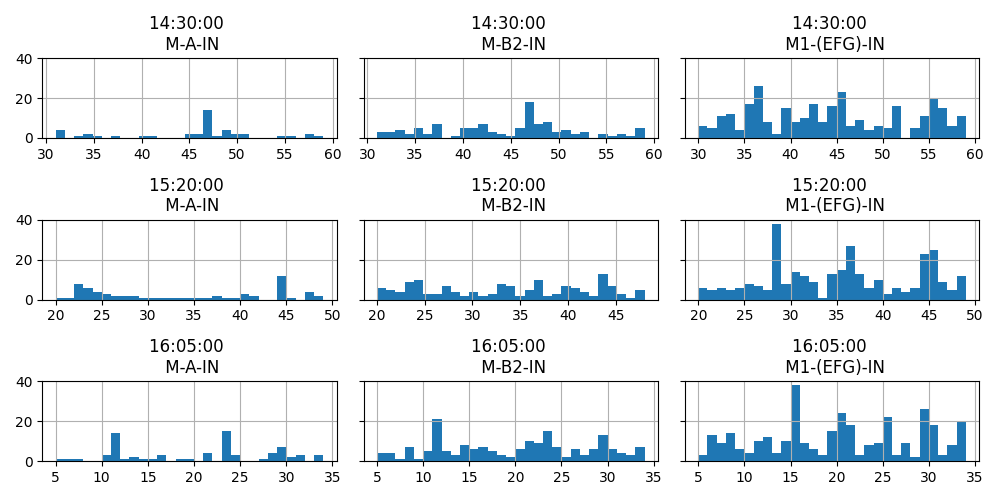
\includegraphics[width=\textwidth]{./appendix/countingExperiment/Day29_IN.png} 
\caption[Counting experiment: pedestrian flows over time]{Counting experiment: pedestrian flows over time}
\label{fig:timeslots}
\end{figure}




\subsection*{Estimating the probability to take the short route}
When people walk from the bus to the metro, the direct short route congestion can occur in the intermediate floor which is not visible at the surface level. I want to know how likely it it is that passengers take the short route and experience congestion. I suggest to estimate the probability from the count data. I assume that the probability to take the short route is the ratio of the flow along the short route and the in-flow:
\begin{equation}
p_{short} = \frac{flow_{short}}{flow_{in}}
\end{equation}
The in-flow is defined as the sum of all flows of arriving passengers at the surface level, that are, arrivals from the bus or tram. I assume that the inflow is  the sum of flows measured at measurement line 1b and 2. Please note that this only holds for a steady state flow and does not consider additional flows from side entrances.

Tab.~\ref{tab:appendixrouteprobscomp} shows the route choice probabilities for the short route. Please be aware that there is uncertainty in this values: there can be other flows involved from side entrances which means the values can be either higher or lower depending on the strength of the unknown side flows. Also, the counting experiment was conducted during a lull in the corona pandemic. This mostly affects the absolute flow values, but I cannot guarantee that it does not shift the distribution of pedestrians over the routes.


%One reason for this is that I can only estimate the route distributions, as no measurement data is available for the passenger flows at bus/tram stations. In addition, the route distribution depends on factors that I cannot control or measure. For example, I know the age and gender distribution from the survey, but not from the measurement data. In addition, I assume that people behave differently under real conditions than they state in the survey. For these reasons, the data are not suitable for validation. The following considerations represent a plausibility check and are not to be equated with a quantitative validation. 



\begin{table}[hbt!]
\begin{tabular}{p{2cm}p{2cm}p{2cm}p{2cm}p{2cm}p{2cm}}
\toprule
Time slot &   M-A-IN &   M-B2-IN &   M1-(EFG)-IN &   M-B-IN-cleaned &  Probability: short route \\
\midrule
14:30:00  &       43 &       111 &           302 &               68 &    0.82 \\
15:20:00  &       65 &       147 &           307 &               82 &    0.79 \\
16:05:00  &       72 &       179 &           329 &              107 &    0.75 \\
\bottomrule
\end{tabular}
\caption[Counting experiment: route probability of the short route for validation]{Counting experiment: route probability of the short route for validation. Total number of arrivals for each time slot and corresponding probability for the short route.}
\label{tab:appendixrouteprobscomp}
\end{table}

Interestingly, the probability of the short route decreases over the number of arrivals, see Fig.~\ref{fig:correlationroutechoice}. This indicates that the more people, the more congestion and the more likely people take alternative routes.  However, I cannot provide statistical evidence with only three data points.

\begin{figure}[hbt!]
\centering
\begin{tikzpicture}
\node[] at (0,0) {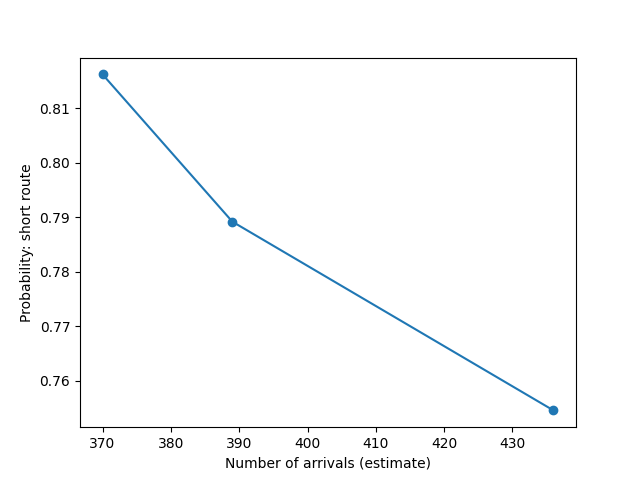
\includegraphics[width=7cm,trim={1cm 0 0 0},clip]{./appendix/countingExperiment/Correlation.png} };
\node[fill=white,font=\small] at (-0.2,-2.5) {370~~~~~~~~390~~~~~~~~410~~~~~~~~430};
\node[fill=white] at (0,-3.2) {Number of arrivals};
\node[fill=white,rotate=90] at (-3.4,0) {Probability: short route };
\node[] at (-2.1,1.9) {0.82};
\node[] at (-0.3,0.4) {0.79};
\node[] at (2.4,-1.4) {0.75};
\end{tikzpicture}
\caption[Estimated probability for the short route over arrivals ]{Estimated probability for the short route over arrivals. The estimated probability to take the short route decreases over the number of arrivals. }
\label{fig:correlationroutechoice}
\end{figure}

\clearpage

\newpage

\thispagestyle{empty}

{\color{white}.}

\vspace{6cm}

\begin{center}
\textit{Last page of the document}
\end{center}




